%==============================================================
%  Figura 8.15 - Dispositivo di arresto di emergenza che agisce
%  sullo sganciatore di minima tensione del dispositivo di
%  sezionamento dell'alimentazione (avviatore motore) (Esempio 7)
%  Adattamento in italiano della Figura 8.15 dell'IFA Report 2/2017
%
%  I simboli riproducono quelli dell'originale: le coordinate sono
%  ricavate dal disegno di partenza (1 cm = 70 px, origine
%  nell'angolo in alto a sinistra della cornice). Nessun cambio di
%  corpo del font: le etichette sono ingrandite con "scale" (vedere
%  la nota nella Figura 8.3). Nell'originale tutti i collegamenti
%  sono in verde scuro e i testi in nero.
%==============================================================
\definecolor{verdepotenza}{RGB}{22,67,38}
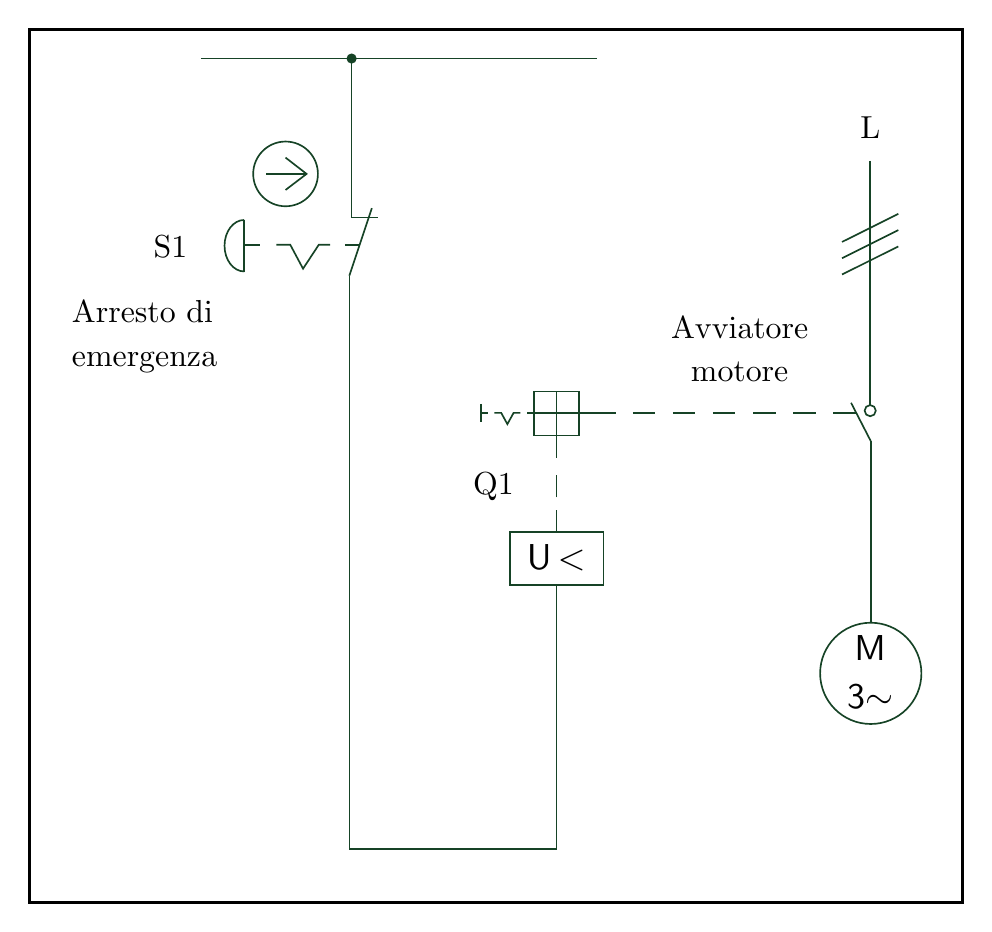
\begin{tikzpicture}[
  font=\normalsize,
  filo/.style={draw=verdepotenza, line width=0.6pt},
  meccanico/.style={draw=verdepotenza, line width=0.6pt, dash pattern=on 0.286cm off 0.223cm},
  etichetta/.style={inner sep=1pt, scale=1.15},
  nodo/.style={circle, fill=verdepotenza, inner sep=0pt, minimum size=0.129cm}
]

%--------------------------------------------------------------
% Cornice
%--------------------------------------------------------------
\draw[draw=black, line width=1.2pt] (0.000,-0.000) rectangle (11.850,-11.086);

%--------------------------------------------------------------
% Linea di alimentazione superiore
%--------------------------------------------------------------
\draw[filo] (2.179,-0.371) -- (7.207,-0.371);
\draw[filo] (4.093,-0.371) -- (4.093,-2.390);
\node[nodo] at (4.093,-0.371) {};

%--------------------------------------------------------------
% S1: dispositivo di arresto di emergenza (pulsante a fungo con
% ritenuta, contatto di apertura ad azionamento meccanico positivo)
%--------------------------------------------------------------
% simbolo di apertura positiva
\draw[filo] (3.254,-1.836) circle (0.411);
\draw[filo] (3.011,-1.836) -- (3.521,-1.836);
\draw[filo] (3.254,-1.629) -- (3.521,-1.836) -- (3.254,-2.040);
% pulsante a fungo
\draw[filo] (2.729,-2.421) -- (2.729,-3.076);
\draw[filo] (2.729,-2.421) arc[start angle=90, end angle=270, x radius=0.250, y radius=0.327];
% collegamento meccanico con ritenuta
\draw[filo] (2.729,-2.736) -- (2.933,-2.736);
\draw[filo] (3.136,-2.736) -- (3.314,-2.736) -- (3.476,-3.040) -- (3.676,-2.736) -- (3.819,-2.736);
\draw[filo] (4.007,-2.736) -- (4.200,-2.736);
% contatto di apertura
\draw[filo] (4.093,-2.390) -- (4.433,-2.390);
\draw[filo] (4.064,-3.129) -- (4.350,-2.271);
\node[etichetta] at (1.793,-2.757) {S1};
\node[etichetta, anchor=base west] at (0.493,-3.729) {Arresto di};
\node[etichetta, anchor=base west] at (0.493,-4.286) {emergenza};

%--------------------------------------------------------------
% Linea di ritorno verso lo sganciatore di minima tensione
%--------------------------------------------------------------
\draw[filo] (4.064,-3.129) -- (4.064,-10.407) -- (6.693,-10.407) -- (6.693,-7.057);

%--------------------------------------------------------------
% Q1: avviatore motore con sganciatore di minima tensione
%--------------------------------------------------------------
\draw[filo] (6.107,-6.386) rectangle (7.293,-7.057);
\node[inner sep=1pt, scale=1.3, font=\sffamily] at (6.693,-6.714) {U\,\textless};
% collegamento meccanico sganciatore - serratura
\draw[filo] (6.693,-6.386) -- (6.693,-6.100);
\draw[filo] (6.693,-5.943) -- (6.693,-5.657);
\draw[filo] (6.693,-5.443) -- (6.693,-4.600);
% serratura
\draw[filo] (6.407,-4.600) rectangle (6.979,-5.157);
\draw[filo] (6.321,-4.871) -- (7.450,-4.871);
% ritenuta a sinistra della serratura
\draw[filo] (5.736,-4.757) -- (5.736,-4.986);
\draw[filo] (5.736,-4.871) -- (5.821,-4.871);
\draw[filo] (5.907,-4.871) -- (5.993,-4.871) -- (6.071,-5.014) -- (6.150,-4.871) -- (6.236,-4.871);
% collegamento meccanico verso il contatto principale
\draw[meccanico] (7.664,-4.871) -- (10.493,-4.871);
\node[etichetta] at (5.893,-5.814) {Q1};
\node[etichetta] at (9.021,-3.786) {Avviatore};
\node[etichetta] at (9.021,-4.343) {motore};

%--------------------------------------------------------------
% Circuito di potenza: linea trifase L, contatto principale di Q1
% e motore M
%--------------------------------------------------------------
\draw[filo] (10.679,-1.671) -- (10.679,-4.771);
\draw[filo] (10.321,-2.700) -- (11.036,-2.343);
\draw[filo] (10.321,-2.907) -- (11.036,-2.550);
\draw[filo] (10.321,-3.114) -- (11.036,-2.757);
\node[etichetta] at (10.679,-1.243) {L};
% contatto principale con apertura automatica
\draw[filo] (10.679,-4.843) circle (0.071);
\draw[filo] (10.436,-4.743) -- (10.686,-5.229);
\draw[filo] (10.686,-5.229) -- (10.686,-7.536);
% motore trifase
\draw[filo] (10.686,-8.179) circle (0.643);
\node[inner sep=1pt, scale=1.3, font=\sffamily] at (10.679,-7.857) {M};
\node[inner sep=1pt, scale=1.3, font=\sffamily] at (10.679,-8.471) {3$\sim$};

\end{tikzpicture}
